\documentclass[final,hyperref={pdfpagelabels=false}]{beamer}
\mode<presentation>{\usetheme[simple_logo]{chalmersposter}}

  \usepackage{times}
  \usepackage{amsmath,amsthm, amssymb, latexsym}
  \boldmath
  \usepackage[english]{babel}
  \usepackage{siunitx}
  \usepackage[utf8]{inputenc}
  \usepackage{graphicx}
  \usepackage{subcaption}
  \usepackage[orientation=portrait ,size=a0,scale=1.4,debug]{beamerposter}
  \usepackage[authoryear, round]{natbib}
  %%%%%%%%%%%%%%%%%%%%%%%%%%%%%%%%%%%%%%%%%%%%%%%%%%%%%%%%%%%%%%%%%%%%%%%%%%%%%%%%%5
  \title{A combined RADAR/passive MW and sub-MM \\ cloud retrieval}
  \author{\vspace{-1cm}\textbf{Simon Pfreundschuh}$^1$, Patrick Eriksson$^1$, David Duncan$^1$,
    Robin Ekelund$^1$, Stuart Fox$^2$, Florian Ewald $^3$, Stefan Bühler$^4$, Manfred Brath$^4$}
  \contactauthor{Simon Pfreundschuh}
  \authormail{simon.pfreundschuh@chalmers.se}
  \institute{$^1$Chalmers University of Technology \\
    $^2$Met Office \\
    $^3$Ludwig-Maximilian Univiersität München \\
    $^4$Universität Hamburg}
  \date{2019-02-18}

  \setbeamerfont{institute in headline}{series = \mdseries, size = \normalsize}

  %%%%%%%%%%%%%%%%%%%%%%%%%%%%%%%%%%%%%%%%%%%%%%%%%%%%%%%%%%%%%%%%%%%%%%%%%%%%%%%%%5
  \begin{document}
  \begin{frame}
    \vspace{-3.5cm}
    \begin{columns}[t]
      \begin{column}{.48\linewidth}

%%%%%%%%%%%%%%%%%%%%%%%%%%%%%%%%%%%%%%%%%%%%%%%%%%%%%%%%%%%%%%%%%%%%%%%%%%%%%%%%
% Abstract
%%%%%%%%%%%%%%%%%%%%%%%%%%%%%%%%%%%%%%%%%%%%%%%%%%%%%%%%%%%%%%%%%%%%%%%%%%%%%%%%
          
        \begin{block}{Abstract}

          \begin{itemize}
          \item Cloud properties are retrieved from combined RADAR,
                passive microwave and passive sub-millimetre observations
          \item Some sentence to make the results sound good
          \end{itemize}
                  
          \vspace{1em}


        \end{block}

%%%%%%%%%%%%%%%%%%%%%%%%%%%%%%%%%%%%%%%%%%%%%%%%%%%%%%%%%%%%%%%%%%%%%%%%%%%%%%%%
% Joint flight campaign
%%%%%%%%%%%%%%%%%%%%%%%%%%%%%%%%%%%%%%%%%%%%%%%%%%%%%%%%%%%%%%%%%%%%%%%%%%%%%%%%
          
        \begin{block}{Joint flight}

          \begin{minipage}[t]{0.6\textwidth}
            \vspace{0pt}
            \begin{itemize}
            \item Joint flight of HALO, Falcon and FAAM aircraft as part of the
              North Atlantic Waveguide and Downstream Impace Experiment (NAWDEX)
              on 14th of October 2016
            \end{itemize}
            \begin{minipage}[b]{0.4\textwdith}
              \vspace{0pt}
              \rule{0pt}{5cm}
            \end{minipage}\hfill%
            \begin{minipage}[b]{0.5\textwidth}
              \vspace{1cm}
              \begin{figure}
              \caption{Flight path of the joint flight campaign  north west of Scotland.}
              \end{figure}
            \end{minipage}
          \end{minipage}%
          \begin{minipage}[t]{0.38\textwidth}
            \vspace{-2cm}
            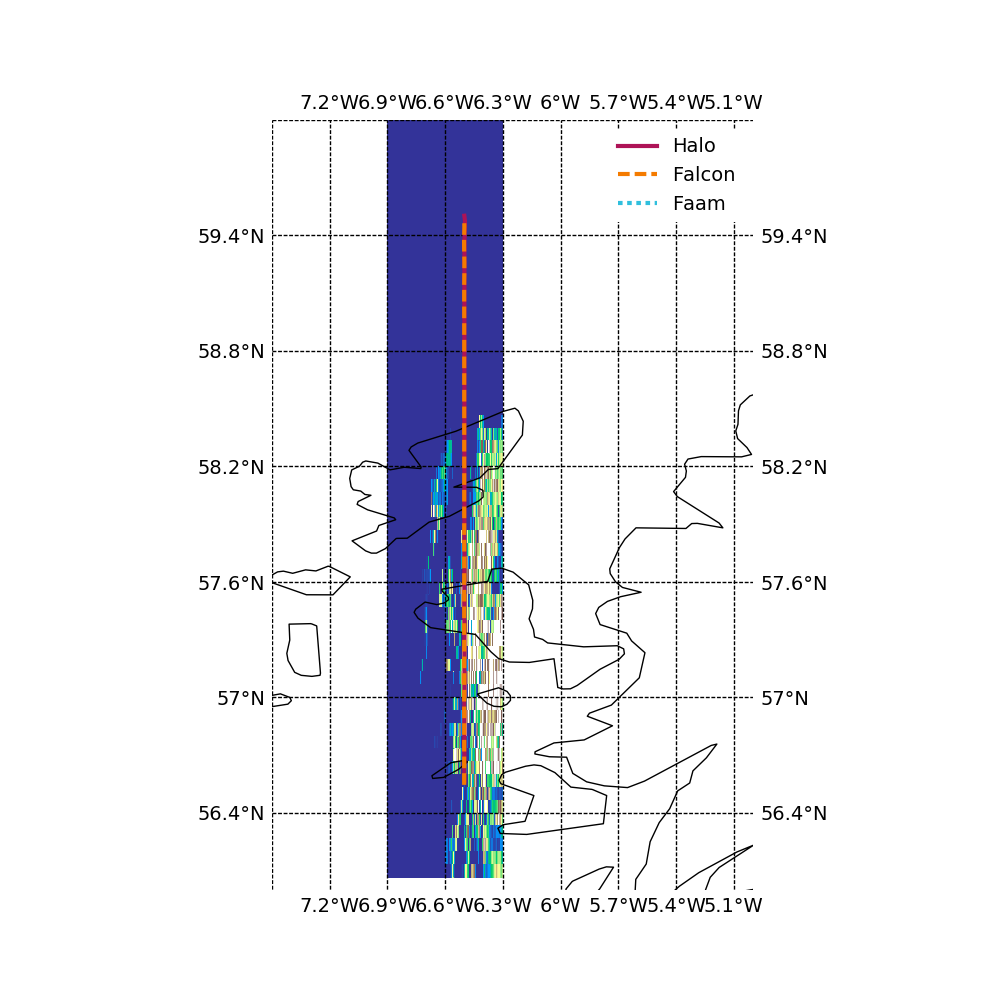
\includegraphics[width=1.0\textwidth]{../plots/flight_path.png}
          \end{minipage}%

           \textbf{Observations}

            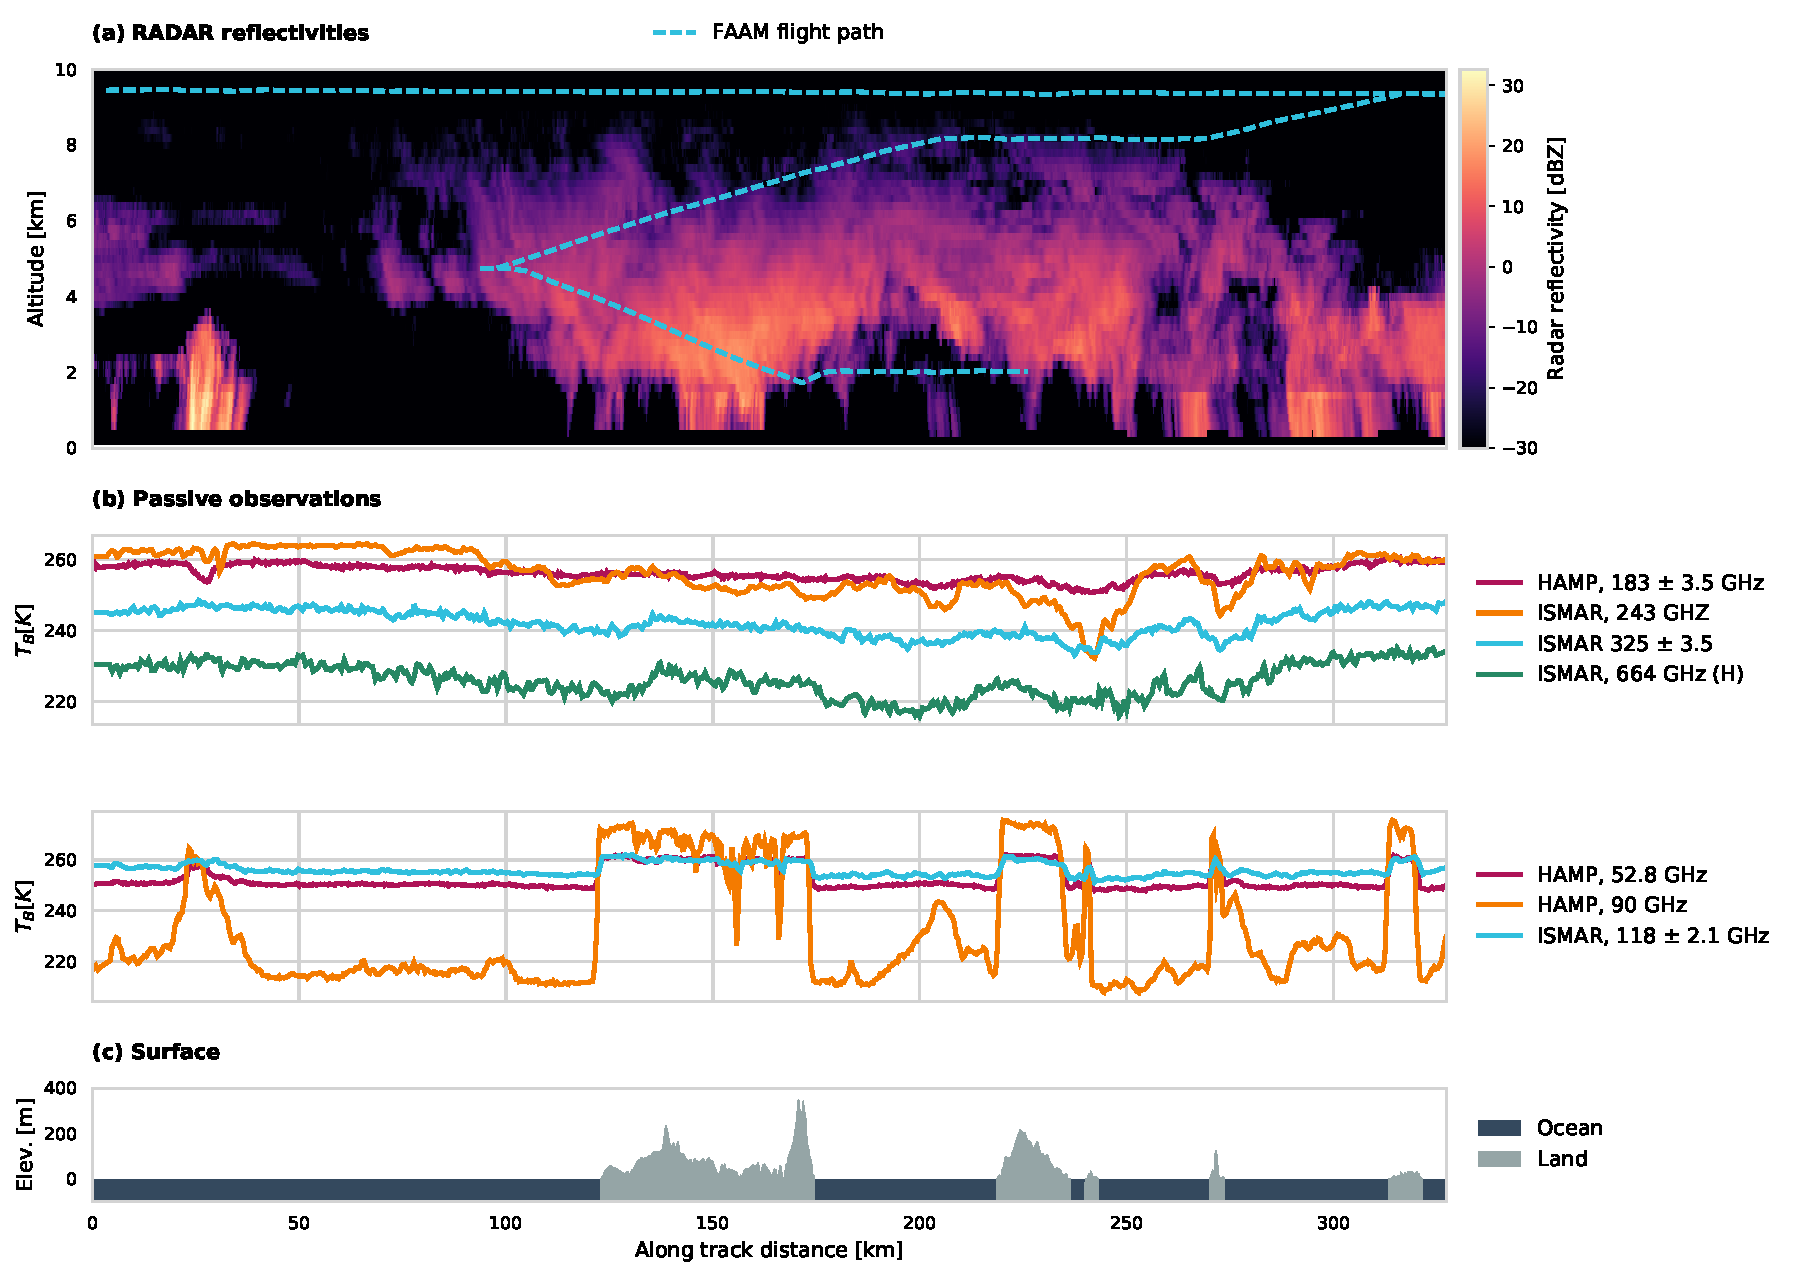
\includegraphics[width=1.0\textwidth]{../plots/observations_combined}
            \begin{figure}
            \centering
            \caption{The combined observations used in the cloud retrieval. Panel (a) shows
              the measured RADAR reflectivity. Panels (b) displays a selection of the micro-
              and sub-mm wave channels used in the retrieval. Panel (c) shows the surface
              type and surface elevation along the flight path.}
            \end{figure}
        \end{block}

%%%%%%%%%%%%%%%%%%%%%%%%%%%%%%%%%%%%%%%%%%%%%%%%%%%%%%%%%%%%%%%%%%%%%%%%%%%%%%%%
% Combined retrieval
%%%%%%%%%%%%%%%%%%%%%%%%%%%%%%%%%%%%%%%%%%%%%%%%%%%%%%%%%%%%%%%%%%%%%%%%%%%%%%%%
          
        \vspace{-2cm}
        \begin{block}{Combined cloud retrieval}

          \begin{itemize}
          \item \textbf{Method}: OEM using ARTS  \citep{arts} as forward model
          \item \textbf{Retrieval targets}: Frozen hydrometeors (1 or 2 species
            depending on settings), Liquid hydrometeors (2 species), Humidity
          \item \textbf{Observations}: HAMP RADAR, HAMP passive microwave, 
               ISMAR passive observations
          \end{itemize}\\[1cm]

          \begin{minipage}[b]{0.6\textwidth}
          \textbf{Microphysics}
           \begin{itemize}
             \item Scattering properties:  ARTS SSDB \citep{arts_ssdb}
             \item PSD: Normalized gamma distribution \citep{delanoe}
           \end{itemize}
           \vfill
           \vspace{2cm}
           \begin{figure}
             \centering
           \begin{minipage}{0.8\textwidth}
             \begin{minipage}{0.5\textwidth}
               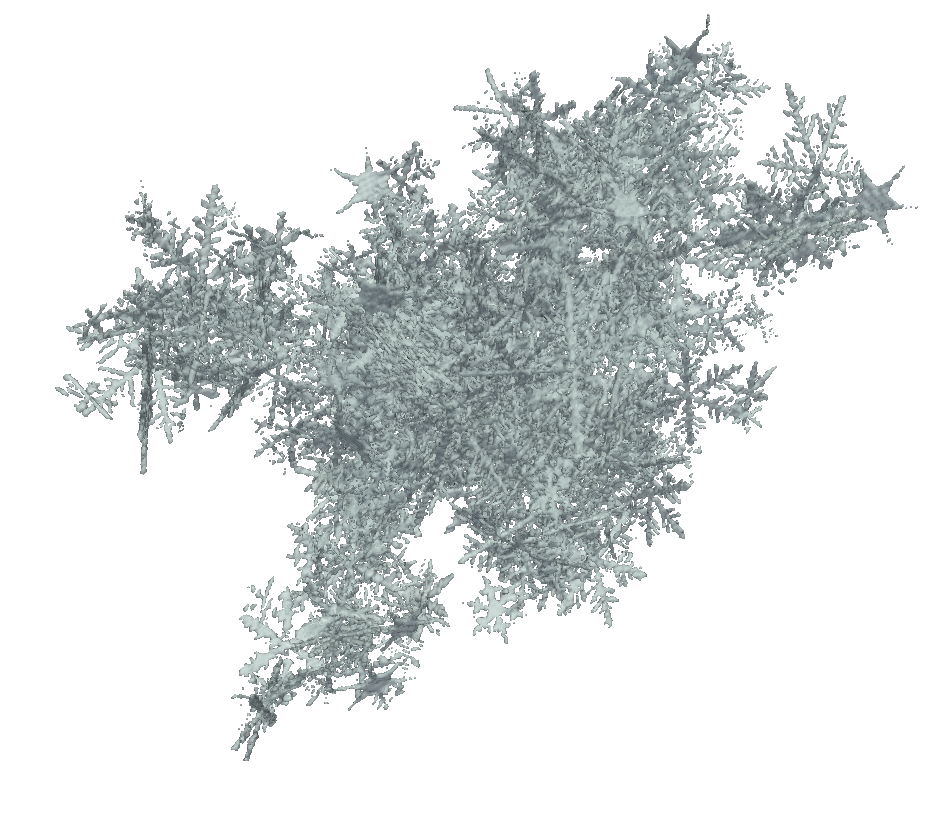
\includegraphics[width = 0.6\textwidth]{../plots/evans_snow_aggregate}
             \end{minipage}\hfill%
             \begin{minipage}{0.5\textwidth}
               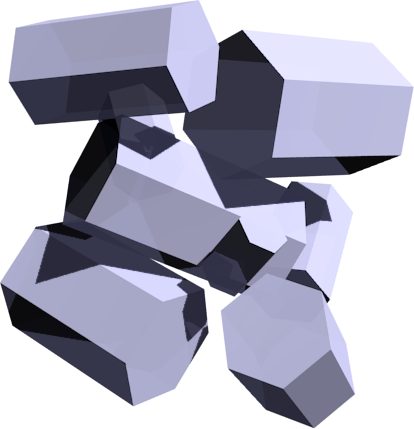
\includegraphics[width = 0.6\textwidth]{../plots/8column_aggregate}
             \end{minipage}
           \end{minipage}
           % caption is wrong.
           \caption{Ice shapes used in the cloud retrieval: 8-ColumnAggregate (left)
                    and Evans snow aggregate (right).}
           \end{figure}
          \end{minipage}%
          \begin{minipage}[b]{0.5\textwidth}
            \begin{figure}
              \centering
              % remove psds
              \includegraphics[width = 0.6\textwidth]{../plots/psds}
              \caption{Shapes of the normalized particles size distributions
                       used in the retrieval.}
             \end{figure}
          \end{minipage}

        \end{block}

    \end{column}

%%%%%%%%%%%%%%%%%%%%%%%%%%%%%%%%%%%%%%%%%%%%%%%%%%%%%%%%%%%%%%%%%%%%%%%%%%%%%%%%
% Results
%%%%%%%%%%%%%%%%%%%%%%%%%%%%%%%%%%%%%%%%%%%%%%%%%%%%%%%%%%%%%%%%%%%%%%%%%%%%%%%%
          
    \begin{column}{.48\linewidth}

      \begin{block}{Results}
      \end{block}

      \begin{block}{Validation}
      \end{block}

      \begin{block}{Conclusions}
      \end{block}

      \begin{block}{Acknowledgements}
      \end{block}

      \begin{block}{References}
        \bibliographystyle{abbrvnat}
        \setcitestyle{authoryear,open={((},close={))}}
        \bibliography{literature}
      \end{block}

    \end{column}
   \end{columns}
  \end{frame}
\end{document}
